\documentclass[12pt,letterpaper]{article}

\usepackage[letterpaper,left=28mm,right=28mm,top=8mm,bottom=0mm]{geometry}
\usepackage{color}
\usepackage{amsmath}
\usepackage{tikz}

%%%%%%%%%%%%%

\newcommand{\digitbox}{%
  \fbox{
  \rule[-1.5ex]{0pt}{4ex}
  \hspace{2ex}}}

\newcommand{\bigdigitbox}{%
  \fbox{
  \rule[-2ex]{0pt}{5ex}
  \hspace{3ex}}}

\pagestyle{empty}

\begin{document}

\begin{center}
  \textbf{Only 1 question per page!}
\end{center}

\begin{flushleft}
\noindent
Test \# \fbox{\digitbox\,\digitbox\,\digitbox\,\digitbox}
  \quad
Student \# \fbox{\digitbox\,\digitbox\,\digitbox\,\digitbox\,%
                    \digitbox\,\digitbox\,\digitbox\,\digitbox}
   \\[1ex]
\noindent
\phantom{est}Q.\#  \fbox{\bigdigitbox\,\bigdigitbox}
\quad
Name: \fbox{ \rule[-2.5ex]{0pt}{6ex}\hspace{52ex} }
\end{flushleft}


\hrule

\vfill

\hrule
\begin{center}
  \textbf{If you need more space, use back or another sheet.}
\end{center}


\begin{tikzpicture}[remember picture,overlay]
  \node[anchor=north west] at (current page.north west) {
    \begin{tikzpicture}
      \coordinate (a) at (0,0);
      \coordinate (b) at (3,0);
      \coordinate (c) at (0,-3);
      \filldraw[draw=black, fill=gray!30] (a)--(b)--(c)--(a);
    \end{tikzpicture}
  };
  \node[anchor=north east] at (current page.north east) {
    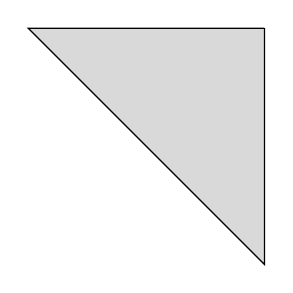
\begin{tikzpicture}
      \coordinate (a) at (0,0);
      \coordinate (b) at (-3,0);
      \coordinate (c) at (0,-3);
      \filldraw[draw=black, fill=gray!30] (a)--(b)--(c)--(a);
    \end{tikzpicture}
  };
  \node[anchor=south west] at (current page.south west) {
    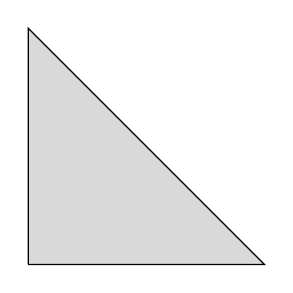
\begin{tikzpicture}
      \coordinate (a) at (0,0);
      \coordinate (b) at (3,0);
      \coordinate (c) at (0,3);
      \filldraw[draw=black, fill=gray!30] (a)--(b)--(c)--(a);
    \end{tikzpicture}
  };
  \node[anchor=south east] at (current page.south east) {
    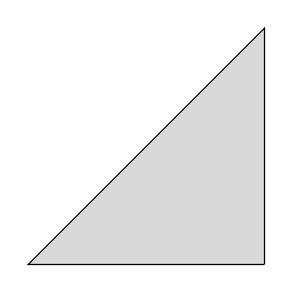
\begin{tikzpicture}
      \coordinate (a) at (0,0);
      \coordinate (b) at (-3,0);
      \coordinate (c) at (0,3);
      \filldraw[draw=black, fill=gray!30] (a)--(b)--(c)--(a);
    \end{tikzpicture}
  };
\end{tikzpicture}


%%%%%%%%%%%%%%%%%%%%%%%%%%%%%%%%%%%%%%%%%%%%%%%%%%%%%%%%%%%%%%%%%%%%%%%%
\clearpage
% Now same again to help ensure people print it double-sided
%%%%%%%%%%%%%%%%%%%%%%%%%%%%%%%%%%%%%%%%%%%%%%%%%%%%%%%%%%%%%%%%%%%%%%%%


\begin{flushleft}
\noindent
Test \# \fbox{\digitbox\,\digitbox\,\digitbox\,\digitbox}
  \quad
Student \# \fbox{\digitbox\,\digitbox\,\digitbox\,\digitbox\,%
                    \digitbox\,\digitbox\,\digitbox\,\digitbox}
   \\[1ex]
\noindent
\phantom{est}Q.\#  \fbox{\bigdigitbox\,\bigdigitbox}
\quad
Name: \fbox{ \rule[-2.5ex]{0pt}{6ex}\hspace{52ex} }
\end{flushleft}

\begin{center}
  \textbf{Only 1 question per page! If you need more space, use back or another sheet.}
\end{center}

\hrule

\vfill

\hrule


\end{document}
